\chapter{Introduction}
In 2014 there were about 800 confirmed exoplanets and more than 3,000 candidates \cite{madhusudhan2014exoplanetary}. Currently these numbers have increased to more than 4,000 conformations and more than 3,750 NASA candidates \cite{nasa_2015}.  Moreover, with the launch of the ARIEL Space Mission from the European Space Agency (ESA) and the launch of the James Webb Space Telescope (JWST) from NASA on the horizon, the census count of exoplanets is expected to drastically increase once these telescopes are in operation. These numbers are relatively small considering that on average each star has a planetary system \cite{krijt2015grains}. The launch of ARIEL and JWST makes the future of exoplanet science look particularly bright. The last two decades in exoplanet science have provided an insight into the properties of exoplanets like mass, radii, temperatures, orbital parameters, C/O ratio and molecular abundances from e.g. $\mathrm{H_2O}$, Na and K \cite{madhusudhan2014exoplanetary, sing2016continuum}. These properties appear to be extremely diverse, so diverse that e.g. the solar system only covers a tiny fraction of the available parameter ranges. It is to be noted that this census consists of exoplanets within the solar neighbourhood \cite{madhusudhan2014exoplanetary}. Fortunately, there is lots more to be discovered, considering the number of observable stars and the fact that each 5th Sun-like star is being orbited by an Earth-like planet \cite{krijt2015grains}. Perhaps it’s only a matter of time until the question of ‘Are we alone?’ is answered. 

Detecting an exoplanet is one thing, detecting atmospheric absorption at different wavelengths from an exoplanet orbiting its host star is a different specialisation. Being able to detect this atmospheric absorption essentially allows for spectroscopy to be performed on the exoplanets atmosphere. In 2014 atmospheric absorption from more than 50 transiting exoplanets and five directly imaged exoplanets have been reported \cite{madhusudhan2014exoplanetary}. In other words, in 2014 an atmospheric absorption spectrum was available for <10\% of the confirmed exoplanets. This does not even comprehend the quality of the data available. The 10-best observed and analysed transmission spectra contain between 17 and 60 spectral bins each \cite{sing2016continuum}. Where each spectral bin measures photons within its wavelength range. These spectra were measured at a wavelength range of 0.3-5 $\mathrm{\mu}$m. The spectra and their fitted atmospheric models are visualised in Figure \ref{fig:nature_spectra}. This fit is created by using a so-called forward model, which is discussed in Chapter \ref{atm_retrieval}. Note that despite the limited spectral resolution, decently looking atmospheric fits have been made. Generally speaking, major advances in the understanding and modelling of exoplanet atmospheres have been made within the last two decades \cite{madhusudhan2014exoplanetary}. 

\begin{figure} [!htb]
    \centering
    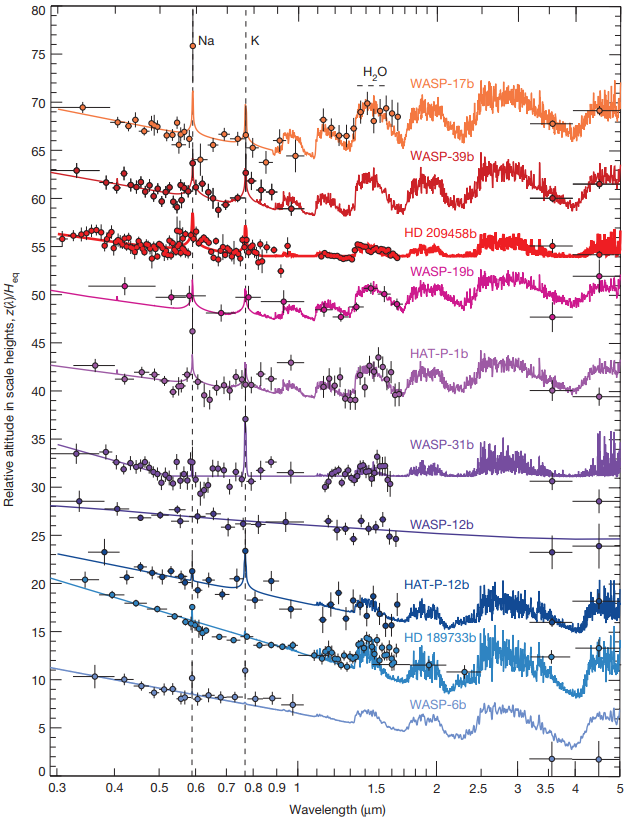
\includegraphics[scale=0.7]{figuren/nature_spectra.png}
    \caption{Hubble Space Telescope and Spitzer transmission measurements for 10 hot-jupiter targets. The solid coloured lines are the fits for the atmospheric models. Horizontal error bars represent the spectral bin, whereas vertical error bars represent the $1
    \sigma$ measurement uncertainty. Figure source: \cite{sing2016continuum}.}
    \label{fig:nature_spectra}
\end{figure}

The detection of atmospheric absorption allows for, but is not limited to, constrains on the chemical composition, temperature and pressure profile, equilibrium and non-equilibrium chemistry, presence or absence of clouds or hazes, and the energy distribution within the atmosphere \cite{madhusudhan2014exoplanetary, madhusudhan2018atmospheric, sing2016continuum, waldmann2015tau}. In return these constrains allow for the interior composition to be constrained and insights into the formation conditions and evolutionary history are gained \cite{benneke2012atmospheric}. The number of free parameters to model exoplanet atmospheres using forward models typically approaches the number of data points available \cite{madhusudhan2018atmospheric}. This results into the need to use statistically robust frameworks. The ARCiS framework for exoplanet atmospheres is an example of such a tool. Two key aspects of ARCiS are accounting for clouds and focusing on the link between planet formation, planet history and the resulting atmospheric composition of the planet \cite{min2019arcis}.

Such realistic and therefor complex frameworks require complex, time-consuming and computationally intensive algorithms to perform an atmospheric retrieval. These frameworks often compare thousands to millions of atmospheric models to the observational data, after which they return the associated model parameters and uncertainties of the best fit \cite{soboczenski2018bayesian, zingales2018exogan}. Runtimes of traditional retrieval models, which mainly make use of Bayesian statistics, scale with the amount of model parameters used \cite{soboczenski2018bayesian}. Recent advances in Machine Learning (ML), or more specifically Deep Learning (DL), offer new ways to reduce the time and computational power required to perform an atmospheric retrieval \cite{waldmann2016dreaming, zingales2018exogan, soboczenski2018bayesian, marquez2018supervised}. It is to be noted that these methods do require a large enough dataset to train on. Generating such a dataset requires a considerable amount of computational power. For most types of neural networks a training sample size of at least 5,000 to 100,000 atmospheric models is required. To put this into perspective, generating 100,000 atmospheric models with ARCiS requires about 6,000 CPU core hours. This equals 9 weeks of full utilisation of a moderate desktop computer. However, once the DL model has been successfully trained, this does result in models being able to perform a retrieval in a matter of seconds to minutes, instead of hundreds to thousands of CPU core hours \cite{soboczenski2018bayesian, zingales2018exogan, marquez2018supervised}.


Deep learning has been used for advances within the field of exoplanets for the last couple of years. It has started with automating the selection process of the parameters to be retrieved in a traditional retrieval \cite{waldmann2016dreaming}. This method aims to minimise the computational power required for a traditional retrieval, due to minimising the number of parameters to be retrieved. Currently this has advanced to performing full retrievals of both physically simple models and more physically complex models \cite{zingales2018exogan, soboczenski2018bayesian}. However, the focus of these methods has been to retrieve the bulk parameters like the planet mass and temperature-pressure profile, together with the abundances of 3 to 12 molecules. With ARIEL and JWST on the horizon, a larger wavelength window and higher spectral resolution will be available \cite{gardner2006james, tinetti2016science}. This results in more data and furthermore, higher quality data coming available. Enabling the search for biosignatures in more detail. Resulting in more molecules to be retrieved, increasing the number of parameters used and therefor increasing the computational power required. Combine this with the increased speed of data coming available and a significant issue appears in terms of computational power. Resulting in compromises having to be made between the detail and run-time of retrievals. To combat this, advances must be made within the field of exoplanet science. Particularly in decreasing the computational power required for a retrieval.

A promising development is ExoGAN \cite{zingales2018exogan}. ExoGAN uses a Deep Convolutional Generative Adversarial Network (DCGAN) which is able to learn the characteristics of atmospheric models, i.e. it learns how transmission spectra of exoplanets look like and what their corresponding parameters and features are. ExoGAN has the ability to perform a retrieval in a matter of seconds to minutes \cite{zingales2018exogan}, instead of the traditional hundreds to thousands of hours. The models generative ability allows for dealing with missing data in a convenient way. Which is fortunate, considering the number of spectral bins available and their diversity in wavelengths, as seen in Figure \ref{fig:nature_spectra}. This diversity in the ranges of the spectral bins is due to measurements being made with different instruments. Combining these two characteristics leads to a difficulty when training traditional neural networks. Often neural networks are designed to take the complete input sequence in a pre-defined format, e.g. the spectral bins of a single instrument. If a traditional neural network is trained on inputs in the form of $[F(\lambda_1),F(\lambda_2),F(\lambda_3),F(\lambda_4),F(\lambda_5)]$, problems will occur when e.g. the value of $F(\lambda_3)$ is an unknown value. Here $F(\lambda_n)$ is the transit depth of the spectral bin $\lambda_n$. ExoGAN is not able to do this. ExoGAN is able to process any measurements within a wavelength of 1$\mu$m to 50$\mu$m, as long as they have a spectral resolution of $R$=100. This allows for the analysis of measurements taken with all kinds of instruments, whether they contain missing data or not. This alone is an advantage, considering that no separate neural networks are required for each individual instrument.
In theory the networks generative ability allows for a significant speed up in forward modelling, considering that it could be used to generate atmospheric models in a matter of seconds to minutes. This concept has been applied in \cite{yip2019pushing}, where a DCGAN is used to generate a synthetic dataset to subsequently train a Convolutional Neural Network (CNN) classifier for the detection of planets.

As promising as ExoGAN is, there is lots of room for improvement. ExoGAN has been trained on a dataset of $10^7$ atmospheric models \cite{zingales2018exogan}. These atmospheric models are created with 7 parameters, the planet mass, planet radius, planet temperature and the abundances of H$_2$O, CO$_2$, CO and CH$_4$. Each parameter has been sampled in 10 bins within a given range \cite{zingales2018exogan}, i.e. they are sampled with discrete values. The spectra are sampled with a wavelength from 1$\mu$m to 50$\mu$m and the forward modelling technique used contains little physics and no chemistry. There are more possibilities for improvement, these are discussed in Chapter 2 \& 3.

Taking the research performed by \cite{zingales2018exogan} and improving it is the main goal of this work. This leads to the research outlines of SRON-GAN. Trivial ways of improvement are listed below.


\begin{itemize}
\item Decrease the amount of training data required by at least an order of magnitude.
\item Sample the atmospheric model parameters continuous, instead of discrete.
\item Decrease the wavelength range from (1-50)$\mu$m to (0.3-16)$\mu$m.
\item Use a dataset which is sampled by using complex physical and chemical models, using ARCiS.
\end{itemize}
This all generalises to the research question; Can we develop a GAN, which is trained on a relatively small sample size of complex physical atmospheric models, and still have it converge?


Summarised, SRON-GAN is a GAN which together with semantic image inpainting performs a retrieval using physical complex models on the transmission spectra of exoplanets. A simple version SRON-GAN will be trained on $10^6$ spectra generated from simple physical models, to validate the networks capability to learn. After which SRON-GAN is trained on $28\cdot10^3$ complex physical models and tested on $12\cdot10^3$ complex physical models. These complex physical models include molecular chemistry, self consistent temperature-pressure profile, and cloud formation. Once SRON-GAN is trained, it will be able to retrieve all the parameters it has been trained on from observed transmission spectra in a matter of seconds.